
%% bare_conf.tex
%% V1.3
%% 2007/01/11
%% by Michael Shell
%% See:
%% http://www.michaelshell.org/
%% for current contact information.
%%
%% This is a skeleton file demonstrating the use of IEEEtran.cls
%% (requires IEEEtran.cls version 1.7 or later) with an IEEE conference paper.
%%
%% Support sites:
%% http://www.michaelshell.org/tex/ieeetran/
%% http://www.ctan.org/tex-archive/macros/latex/contrib/IEEEtran/
%% and
%% http://www.ieee.org/

%%*************************************************************************
%% Legal Notice:
%% This code is offered as-is without any warranty either expressed or
%% implied; without even the implied warranty of MERCHANTABILITY or
%% FITNESS FOR A PARTICULAR PURPOSE! 
%% User assumes all risk.
%% In no event shall IEEE or any contributor to this code be liable for
%% any damages or losses, including, but not limited to, incidental,
%% consequential, or any other damages, resulting from the use or misuse
%% of any information contained here.
%%
%% All comments are the opinions of their respective authors and are not
%% necessarily endorsed by the IEEE.
%%
%% This work is distributed under the LaTeX Project Public License (LPPL)
%% ( http://www.latex-project.org/ ) version 1.3, and may be freely used,
%% distributed and modified. A copy of the LPPL, version 1.3, is included
%% in the base LaTeX documentation of all distributions of LaTeX released
%% 2003/12/01 or later.
%% Retain all contribution notices and credits.
%% ** Modified files should be clearly indicated as such, including  **
%% ** renaming them and changing author support contact information. **
%%
%% File list of work: IEEEtran.cls, IEEEtran_HOWTO.pdf, bare_adv.tex,
%%                    bare_conf.tex, bare_jrnl.tex, bare_jrnl_compsoc.tex
%%*************************************************************************

% *** Authors should verify (and, if needed, correct) their LaTeX system  ***
% *** with the testflow diagnostic prior to trusting their LaTeX platform ***
% *** with production work. IEEE's font choices can trigger bugs that do  ***
% *** not appear when using other class files.                            ***
% The testflow support page is at:
% http://www.michaelshell.org/tex/testflow/



% Note that the a4paper option is mainly intended so that authors in
% countries using A4 can easily print to A4 and see how their papers will
% look in print - the typesetting of the document will not typically be
% affected with changes in paper size (but the bottom and side margins will).
% Use the testflow package mentioned above to verify correct handling of
% both paper sizes by the user's LaTeX system.
%
% Also note that the "draftcls" or "draftclsnofoot", not "draft", option
% should be used if it is desired that the figures are to be displayed in
% draft mode.
%
\documentclass[conference]{IEEEtran}
\usepackage{blindtext, graphicx}
\usepackage{hyperref}
\usepackage{multirow}
% Add the compsoc option for Computer Society conferences.
%
% If IEEEtran.cls has not been installed into the LaTeX system files,
% manually specify the path to it like:
% \documentclass[conference]{../sty/IEEEtran}





% Some very useful LaTeX packages include:
% (uncomment the ones you want to load)


% *** MISC UTILITY PACKAGES ***
%
%\usepackage{ifpdf}
% Heiko Oberdiek's ifpdf.sty is very useful if you need conditional
% compilation based on whether the output is pdf or dvi.
% usage:
% \ifpdf
%   % pdf code
% \else
%   % dvi code
% \fi
% The latest version of ifpdf.sty can be obtained from:
% http://www.ctan.org/tex-archive/macros/latex/contrib/oberdiek/
% Also, note that IEEEtran.cls V1.7 and later provides a builtin
% \ifCLASSINFOpdf conditional that works the same way.
% When switching from latex to pdflatex and vice-versa, the compiler may
% have to be run twice to clear warning/error messages.






% *** CITATION PACKAGES ***
%
\usepackage{cite}
% cite.sty was written by Donald Arseneau
% V1.6 and later of IEEEtran pre-defines the format of the cite.sty package
% \cite{} output to follow that of IEEE. Loading the cite package will
% result in citation numbers being automatically sorted and properly
% "compressed/ranged". e.g., [1], [9], [2], [7], [5], [6] without using
% cite.sty will become [1], [2], [5]--[7], [9] using cite.sty. cite.sty's
% \cite will automatically add leading space, if needed. Use cite.sty's
% noadjust option (cite.sty V3.8 and later) if you want to turn this off.
% cite.sty is already installed on most LaTeX systems. Be sure and use
% version 4.0 (2003-05-27) and later if using hyperref.sty. cite.sty does
% not currently provide for hyperlinked citations.
% The latest version can be obtained at:
% http://www.ctan.org/tex-archive/macros/latex/contrib/cite/
% The documentation is contained in the cite.sty file itself.






% *** GRAPHICS RELATED PACKAGES ***
%
\ifCLASSINFOpdf
  % \usepackage[pdftex]{graphicx}
  % declare the path(s) where your graphic files are
  % \graphicspath{{../pdf/}{../jpeg/}}
  % and their extensions so you won't have to specify these with
  % every instance of \includegraphics
  % \DeclareGraphicsExtensions{.pdf,.jpeg,.png}
\else
  % or other class option (dvipsone, dvipdf, if not using dvips). graphicx
  % will default to the driver specified in the system graphics.cfg if no
  % driver is specified.
  % \usepackage[dvips]{graphicx}
  % declare the path(s) where your graphic files are
  % \graphicspath{{../eps/}}
  % and their extensions so you won't have to specify these with
  % every instance of \includegraphics
  % \DeclareGraphicsExtensions{.eps}
\fi
% graphicx was written by David Carlisle and Sebastian Rahtz. It is
% required if you want graphics, photos, etc. graphicx.sty is already
% installed on most LaTeX systems. The latest version and documentation can
% be obtained at: 
% http://www.ctan.org/tex-archive/macros/latex/required/graphics/
% Another good source of documentation is "Using Imported Graphics in
% LaTeX2e" by Keith Reckdahl which can be found as epslatex.ps or
% epslatex.pdf at: http://www.ctan.org/tex-archive/info/
%
% latex, and pdflatex in dvi mode, support graphics in encapsulated
% postscript (.eps) format. pdflatex in pdf mode supports graphics
% in .pdf, .jpeg, .png and .mps (metapost) formats. Users should ensure
% that all non-photo figures use a vector format (.eps, .pdf, .mps) and
% not a bitmapped formats (.jpeg, .png). IEEE frowns on bitmapped formats
% which can result in "jaggedy"/blurry rendering of lines and letters as
% well as large increases in file sizes.
%
% You can find documentation about the pdfTeX application at:
% http://www.tug.org/applications/pdftex





% *** MATH PACKAGES ***
%
\usepackage[cmex10]{amsmath}
% A popular package from the American Mathematical Society that provides
% many useful and powerful commands for dealing with mathematics. If using
% it, be sure to load this package with the cmex10 option to ensure that
% only type 1 fonts will utilized at all point sizes. Without this option,
% it is possible that some math symbols, particularly those within
% footnotes, will be rendered in bitmap form which will result in a
% document that can not be IEEE Xplore compliant!
%
% Also, note that the amsmath package sets \interdisplaylinepenalty to 10000
% thus preventing page breaks from occurring within multiline equations. Use:
%\interdisplaylinepenalty=2500
% after loading amsmath to restore such page breaks as IEEEtran.cls normally
% does. amsmath.sty is already installed on most LaTeX systems. The latest
% version and documentation can be obtained at:
% http://www.ctan.org/tex-archive/macros/latex/required/amslatex/math/





% *** SPECIALIZED LIST PACKAGES ***
%
%\usepackage{algorithmic}
% algorithmic.sty was written by Peter Williams and Rogerio Brito.
% This package provides an algorithmic environment fo describing algorithms.
% You can use the algorithmic environment in-text or within a figure
% environment to provide for a floating algorithm. Do NOT use the algorithm
% floating environment provided by algorithm.sty (by the same authors) or
% algorithm2e.sty (by Christophe Fiorio) as IEEE does not use dedicated
% algorithm float types and packages that provide these will not provide
% correct IEEE style captions. The latest version and documentation of
% algorithmic.sty can be obtained at:
% http://www.ctan.org/tex-archive/macros/latex/contrib/algorithms/
% There is also a support site at:
% http://algorithms.berlios.de/index.html
% Also of interest may be the (relatively newer and more customizable)
% algorithmicx.sty package by Szasz Janos:
% http://www.ctan.org/tex-archive/macros/latex/contrib/algorithmicx/




% *** ALIGNMENT PACKAGES ***
%
%\usepackage{array}
% Frank Mittelbach's and David Carlisle's array.sty patches and improves
% the standard LaTeX2e array and tabular environments to provide better
% appearance and additional user controls. As the default LaTeX2e table
% generation code is lacking to the point of almost being broken with
% respect to the quality of the end results, all users are strongly
% advised to use an enhanced (at the very least that provided by array.sty)
% set of table tools. array.sty is already installed on most systems. The
% latest version and documentation can be obtained at:
% http://www.ctan.org/tex-archive/macros/latex/required/tools/


%\usepackage{mdwmath}
%\usepackage{mdwtab}
% Also highly recommended is Mark Wooding's extremely powerful MDW tools,
% especially mdwmath.sty and mdwtab.sty which are used to format equations
% and tables, respectively. The MDWtools set is already installed on most
% LaTeX systems. The lastest version and documentation is available at:
% http://www.ctan.org/tex-archive/macros/latex/contrib/mdwtools/


% IEEEtran contains the IEEEeqnarray family of commands that can be used to
% generate multiline equations as well as matrices, tables, etc., of high
% quality.


%\usepackage{eqparbox}
% Also of notable interest is Scott Pakin's eqparbox package for creating
% (automatically sized) equal width boxes - aka "natural width parboxes".
% Available at:
% http://www.ctan.org/tex-archive/macros/latex/contrib/eqparbox/





% *** SUBFIGURE PACKAGES ***
%\usepackage[tight,footnotesize]{subfigure}
% subfigure.sty was written by Steven Douglas Cochran. This package makes it
% easy to put subfigures in your figures. e.g., "Figure 1a and 1b". For IEEE
% work, it is a good idea to load it with the tight package option to reduce
% the amount of white space around the subfigures. subfigure.sty is already
% installed on most LaTeX systems. The latest version and documentation can
% be obtained at:
% http://www.ctan.org/tex-archive/obsolete/macros/latex/contrib/subfigure/
% subfigure.sty has been superceeded by subfig.sty.



%\usepackage[caption=false]{caption}
%\usepackage[font=footnotesize]{subfig}
% subfig.sty, also written by Steven Douglas Cochran, is the modern
% replacement for subfigure.sty. However, subfig.sty requires and
% automatically loads Axel Sommerfeldt's caption.sty which will override
% IEEEtran.cls handling of captions and this will result in nonIEEE style
% figure/table captions. To prevent this problem, be sure and preload
% caption.sty with its "caption=false" package option. This is will preserve
% IEEEtran.cls handing of captions. Version 1.3 (2005/06/28) and later 
% (recommended due to many improvements over 1.2) of subfig.sty supports
% the caption=false option directly:
%\usepackage[caption=false,font=footnotesize]{subfig}
%
% The latest version and documentation can be obtained at:
% http://www.ctan.org/tex-archive/macros/latex/contrib/subfig/
% The latest version and documentation of caption.sty can be obtained at:
% http://www.ctan.org/tex-archive/macros/latex/contrib/caption/




% *** FLOAT PACKAGES ***
%
%\usepackage{fixltx2e}
% fixltx2e, the successor to the earlier fix2col.sty, was written by
% Frank Mittelbach and David Carlisle. This package corrects a few problems
% in the LaTeX2e kernel, the most notable of which is that in current
% LaTeX2e releases, the ordering of single and double column floats is not
% guaranteed to be preserved. Thus, an unpatched LaTeX2e can allow a
% single column figure to be placed prior to an earlier double column
% figure. The latest version and documentation can be found at:
% http://www.ctan.org/tex-archive/macros/latex/base/



%\usepackage{stfloats}
% stfloats.sty was written by Sigitas Tolusis. This package gives LaTeX2e
% the ability to do double column floats at the bottom of the page as well
% as the top. (e.g., "\begin{figure*}[!b]" is not normally possible in
% LaTeX2e). It also provides a command:
%\fnbelowfloat
% to enable the placement of footnotes below bottom floats (the standard
% LaTeX2e kernel puts them above bottom floats). This is an invasive package
% which rewrites many portions of the LaTeX2e float routines. It may not work
% with other packages that modify the LaTeX2e float routines. The latest
% version and documentation can be obtained at:
% http://www.ctan.org/tex-archive/macros/latex/contrib/sttools/
% Documentation is contained in the stfloats.sty comments as well as in the
% presfull.pdf file. Do not use the stfloats baselinefloat ability as IEEE
% does not allow \baselineskip to stretch. Authors submitting work to the
% IEEE should note that IEEE rarely uses double column equations and
% that authors should try to avoid such use. Do not be tempted to use the
% cuted.sty or midfloat.sty packages (also by Sigitas Tolusis) as IEEE does
% not format its papers in such ways.





% *** PDF, URL AND HYPERLINK PACKAGES ***
%
%\usepackage{url}
% url.sty was written by Donald Arseneau. It provides better support for
% handling and breaking URLs. url.sty is already installed on most LaTeX
% systems. The latest version can be obtained at:
% http://www.ctan.org/tex-archive/macros/latex/contrib/misc/
% Read the url.sty source comments for usage information. Basically,
% \url{my_url_here}.





% *** Do not adjust lengths that control margins, column widths, etc. ***
% *** Do not use packages that alter fonts (such as pslatex).         ***
% There should be no need to do such things with IEEEtran.cls V1.6 and later.
% (Unless specifically asked to do so by the journal or conference you plan
% to submit to, of course. )


% correct bad hyphenation here
\hyphenation{op-tical net-works semi-conduc-tor}


\begin{document}
%
% paper title
% can use linebreaks \\ within to get better formatting as desired
\title{Automatic Vehicle Identification and Classification}


% author names and affiliations
% use a multiple column layout for up to three different
% affiliations
\author{\IEEEauthorblockN{Darren Karl A. Sapalo}
\IEEEauthorblockA{College of Computer Studies\\
De La Salle University, Manila\\
2401 Taft Ave, Malate, Manila, 1004 Metro Manila\\
Email: darren\_karl\_sapalo@dlsu.edu.ph}

% \and
% \IEEEauthorblockN{Dr. Joel Ilao}
% \IEEEauthorblockA{College of Computer Studies\\
% De La Salle University, Manila\\
% 2401 Taft Ave, Malate, Manila, 1004 Metro Manila\\
% Email: joel.ilao@delasalle.ph}
}

% make the title area
\maketitle


\begin{abstract}
%\boldmath
This paper presents an automatic vehicle identification and classification system to be able to estimate the volume of vehicular traffic from video sequences. The two primary goals of this research is (1) to be able to classify vehicles commonly found in the Philippines into six classifications: sedan, bus, jeep, truck, SUV, and others; and (2) to be able to estimate the number of vehicles that pass the road. The video processing is done offline (i.e. not in real-time) and relies on manual calibration of lane dividing lines. The primary reference (technical paper) of this automatic traffic surveillance system used two features: size and linearity. This extension research reports design challenges of automatic traffic surveillance systems in the Philippine context and offers its recommendations and opportunities for future work.
\end{abstract}

% Note that keywords are not normally used for peerreview papers.
\begin{IEEEkeywords}
Intelligent traffic systems, image processing, vehicle classification, vehicle counting
\end{IEEEkeywords}






% For peer review papers, you can put extra information on the cover
% page as needed:
% \ifCLASSOPTIONpeerreview
% \begin{center} \bfseries EDICS Category: 3-BBND \end{center}
% \fi
%
% For peerreview papers, this IEEEtran command inserts a page break and
% creates the second title. It will be ignored for other modes.
\IEEEpeerreviewmaketitle

\section{Introduction}
A goal of intelligent transportation systems is to extract traffic information such as traffic density from video streams of traffic \cite{Jun-Wei}. Traffic surveillance systems aim to detect, track, and classify vehicles. Being able to detect and classify vehicles can aid in estimating traffic density and pollution levels in cities and can help traffic enforcers coordinate traffic flow.

\section{Methodology}
The vehicle identification and classification approach is based on the research of \cite{Jun-Wei}.

\subsection{Data Collection}

In this research, there were three (3) RGB video dataset collected, lasting an average of around three (3) minutes using a hand-held Samsung Galaxy S4 smart phone. The initial resolution of the videos were 1920x1080 and were reduced to 480x270. The video datasets were recorded from three places: the first video dataset was collected from the fourth floor of the Gokongwei Building of De La Salle University, Manila (DLSU) facing Taft Avenue. The first dataset covers only one side of the road, with only one general direction of vehicle movement.

\begin{figure}[!h]
\centering
% 
\includegraphics[width=2.5in]{myfigure}
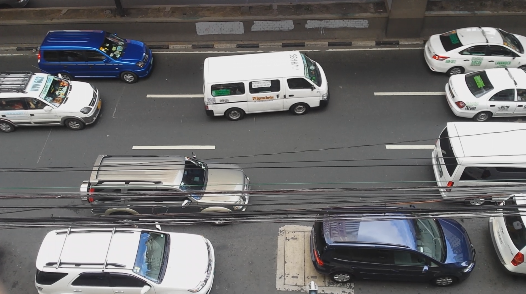
\includegraphics[width=3in]{dataset1_sample.png}
% where an .eps filename suffix will be assumed under latex, 
% and a .pdf suffix will be assumed for pdflatex; or what has been declared
% via \DeclareGraphicsExtensions.
\caption{Problem of occlusion: Electrical cables and parked vehicles in the Gokongwei dataset}
\label{fig_electrical_cables}
\end{figure}

\textbf{Gokongwei Dataset.} The first dataset inherently had problems of occlusion and presented common vehicle behavior based on the location: there were some electrical lines that occluded the road and vehicles and there were also some vehicles that would double-park (parking beside another parked vehicle). Figure~\ref{fig_electrical_cables} shows how the region of interest has been reduced, and how parked vehicles can affect vehicle flow on the road.

\textbf{Buendia Dataset.} The second venue for data collection was on the Light Rail Transit 1, Buendia Station, facing the Makati Central Business District. This dataset was able to capture both sides of the road, capturing two directions of vehicle movement left road (moving downwards) and the right road (moving upwards). This dataset proved to be better than the first one because it did not have the electrical cables that added occlusion. However, because there was an intersection underneath the LRT station, cars on one side of the two roads frequently had stalled vehicles because of the traffic stoplight as seen in figure~\ref{fig_traffic}. This will greatly affect segmentation based on background differencing. Common vehicles in the second dataset are sedans, jeeps, motorcycles, buses, SUVs, trucks, and others, ordered by most frequent to least frequent.


\begin{figure}[!h]
\centering
% 
\includegraphics[width=2.5in]{myfigure}
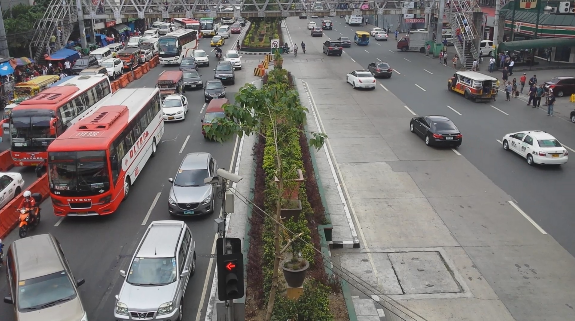
\includegraphics[width=3in]{dataset2_sample.png}
% where an .eps filename suffix will be assumed under latex, 
% and a .pdf suffix will be assumed for pdflatex; or what has been declared
% via \DeclareGraphicsExtensions.
\caption{Problem of stalled vehicles: Traffic has accumulated on the southbound road because of the stoplight in the Buendia dataset}
\label{fig_traffic}
\end{figure}

\begin{figure}[!ht]
\centering
% 
\includegraphics[width=2.5in]{myfigure}
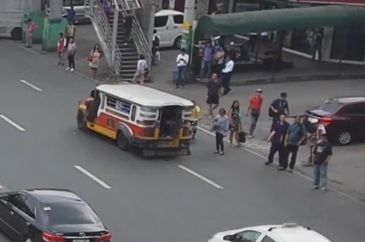
\includegraphics[width=3in]{dataset2_jeeps.png}
% where an .eps filename suffix will be assumed under latex, 
% and a .pdf suffix will be assumed for pdflatex; or what has been declared
% via \DeclareGraphicsExtensions.
\caption{Problem of parked vehicles: Vehicles such as jeeps and buses park on the side of road and in the middle of lanes to load and alight passengers}
\label{fig_jeeps}
\end{figure}

Another issue with this dataset is that jeeps park on the side of the road as seen in figure~\ref{fig_jeeps}.  These parked vehicles waiting for passengers to board and alight will adversely affect the segmentation process. The background modeling module will have erroneous results as vehicles that do not move for a long time are gradually learned as part of the background.

\textbf{EDSA Dataset.} The third venue for data collection was on top of a walkway across EDSA Avenue, near Evangelista Street, Makati City. The video sequence faces northbound with vehicles moving southbound and lasts approximately three minutes for a total of 3567 frames. Common vehicles in the third dataset are sedans, motorcycles, SUVs, jeeps, buses, and trucks, ordered by most frequent to least frequent.


The common vehicles in the Philippines can be categorized as \textit{sedans}, \textit{buses}, \textit{jeeps}, \textit{SUVs}, \textit{trucks}, and \textit{others}. These are the classes used by this system for vehicle classification. An example of these classes are shown in figures~\ref{fig_sedan} to \ref{fig_van}. The \textit{others} class includes vehicles such as motorcycles and vans.


\begin{figure}[!ht]
\centering
% 
\includegraphics[width=2.5in]{myfigure}
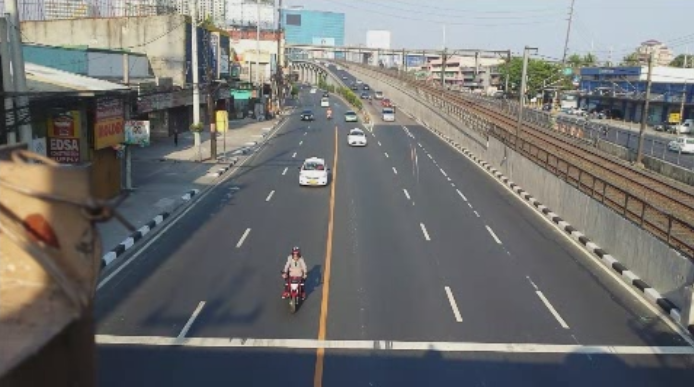
\includegraphics[width=3in]{dataset3_sample.png}
% where an .eps filename suffix will be assumed under latex, 
% and a .pdf suffix will be assumed for pdflatex; or what has been declared
% via \DeclareGraphicsExtensions.
\caption{Vehicles in EDSA Avenue moving southbound. There were no parked or stalled vehicles in this dataset.}
\label{fig_edsa}
\end{figure}

Most of the noise in the traffic dataset was caused either camera movements caused by the hand, or by erroneous re-focusing of the imaging device (Samsung Galaxy S4). Whenever the camera re-focused, there were significant illumination changes in the data. This occurred in tests when using other imaging devices as well (iPhone 5s).

In the study of \cite{Jun-Wei}, shadows were very prominent in their traffic video dataset. They propose a shadow elimination algorithm that replaces the pixel value on the region of interest with the pixel value on the background model if it has a high probability that it is a shadow pixel. The probability of being a shadow pixel was computed based on the mean and variance of shadow pixels acquired from numerous training data on shadows.

\subsection{Stabilization}
First, the video dataset was stabilized so that small camera movements caused by the minimal shaking of the camera can be reduced, if not removed. In the data collection of the EDSA dataset, a makeshift tripod was used to remove small camera movements caused by hand movements.

\subsection{Background Modeling}
Once the video has been stabilized and the movement between frames has been reduced, background modeling can be performed. The video is first converted to grayscale before the background model is acquired. There are various ways to achieve a background model from a video sequence. Initial experiments performed a simple \textbf{weighted background learning approach} to acquire the background model $B_i$ at time $i$:

$$
B_i(x, y) = B_{i-1}(x, y) \cdot (1 - \alpha) \enspace + \enspace I_i(x,y) \cdot \alpha
$$

Majority of the known background model is acquired from the previous background model $B_{i-1}$. The background model learns at a rate of $\alpha$, acquiring only that much information from the current image $I_i$. Various values for $\alpha$ was tested: 0.05, 0.01, 0.005. This produced multiple background models which were manually inspected to evaluate its performance. A higher value for $\alpha$ meant that the background model learned the background faster: non-moving and slow moving objects in the scene will be accepted as the background faster. This proved to be unsuitable for the dataset, as there were slow moving vehicles. However, having too small a value for $\alpha$ meant that it will take longer before the background model is completed. Also, stalled vehicles, which is incorrectly learned as background, will take longer to be unlearned because of the stoplight. Empirical studies showed that the optimal value for $\alpha$ was 0.005.

\subsection{Segmentation By Image Differencing}

After acquiring a sufficient background model, the next step is to perform image differencing between the captured image $I_i$ and the background model $B_i$ to produce the preliminary result of segmentation $D_i$.

$$
D_i(x,y) =  | \enspace I_i(x,y) \enspace - \enspace B_i(x,y) \enspace |
$$

The formula above acquires the distance of the current image $I_i$ to the background model $B_i$ by getting the absolute difference of their values. Afterwards, the binary image which represents the region of interest $R_i$ is acquired by performing thresholding.

$$
R_i(x,y) = \left\{
		\begin{array}{lr}
        1 & D_i(x,y) \geq D \\
        0 & otherwise\\
        \end{array}\right\}
$$

If the value found at $D_i$ is above the average error $D$ then it means that it is part of the foreground. This produces a segmentation mask.

\subsection{Segmentation}

Although initial experiments made use of the simple weighted background learning approach in conjunction with the image differencing, an alternative tool was used to acquire the segmentation mask.

Authors of \cite{Sobral} developed an open source background subtraction library that provides basic to more advanced background subtraction methods. The system is available at \url{https://github.com/andrewssobral/bgslibrary}. The alternative algorithm used for segmentation was the Sigma-Delta background subtraction algorithm by \cite{Manzanera}. The algorithm proved be effective in isolating the vehicles from the background. Figure~\ref{fig_segmentation} shows the segmentation result of a few cars approaching from the distance. A road mask was also applied so that noise outside of the road can be removed.

\begin{figure}[!ht]
\centering
% 
\includegraphics[width=2.5in]{myfigure}
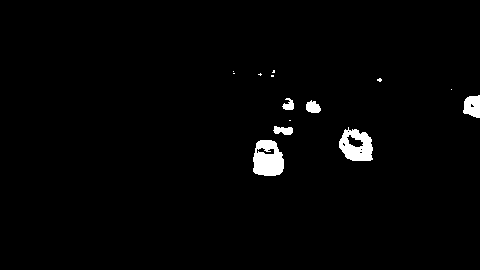
\includegraphics[width=3in]{segmented_mask_sample.png}
% where an .eps filename suffix will be assumed under latex, 
% and a .pdf suffix will be assumed for pdflatex; or what has been declared
% via \DeclareGraphicsExtensions.
\caption{The result of segmentation using the $\Sigma-\Delta$ background subtraction algorithm by \cite{Manzanera}.}
\label{fig_segmentation}
\end{figure}

\subsection{Vehicle identification}

The vehicle identification and classification algorithm used in this research is based on \cite{Jun-Wei}, which makes use of size and linearity as the features for vehicle classification.



The first step in vehicle identification is to detect \textit{Blobs} (the white regions in the mask), acquire their area, and filter the blobs based on their area within a certain threshold. Blobs with area between 500 $\rightarrow$ 15000 were kept as possible vehicles. These values were acquired by analyzing the sizes of vehicles from a far distance and near the video camera. By performing this filtering, we remove the small occurrences of noise seen in figure~\ref{fig_segmentation}.

The second step is to track the movement of the blobs with respect to the previous frame. This allows us to understand what blob in the previous frame is the same blob in the current frame. Doing this allows the system to detect the movement of a vehicle.

The third step is to acquire and normalize the features of the vehicle: size and linearity \cite{Sobral}. The first feature is the \textbf{size feature}, normalized by dividing the area of the blob by the width of the lane dividing lines $W_{Lane_{i}}$ at the centroid of the blob $p$ at lane $i$:

$$
W_{Lane_{i}}(p) = | \quad X_{DL_{i}}(y_p) - X_{DL_{i + 1}}(y_p) \quad |
$$

The width of the lane dividing line is the horizontal distance between two adjacent lane dividing lines $X_{DL_{i}}$ and $X_{DL_{i+1}}$. \cite{Jun-Wei} provides a way to automatically detect lane dividing lines by analyzing a 2D histogram populated by the the positions of the centroids in the blobs in a video sequence. However in this research, the lane dividing lines are manually calibrated. 

The second feature is the \textbf{linearity feature}, which analyzes the up-slanted edges of a vehicle. \cite{Jun-Wei} provides figure~\ref{fig_linearity}, illustrating the concept of linearity. The truck on the left shows low linearity because its up-slanted edges has missing parts in the blob. On the other hand, the up-slanted edges of the bus fits perfectly on a straight line with minimal error, however it has some useless boundary points on the right side of the blob.


\begin{figure}[!ht]
\centering
% 
\includegraphics[width=2.5in]{myfigure}
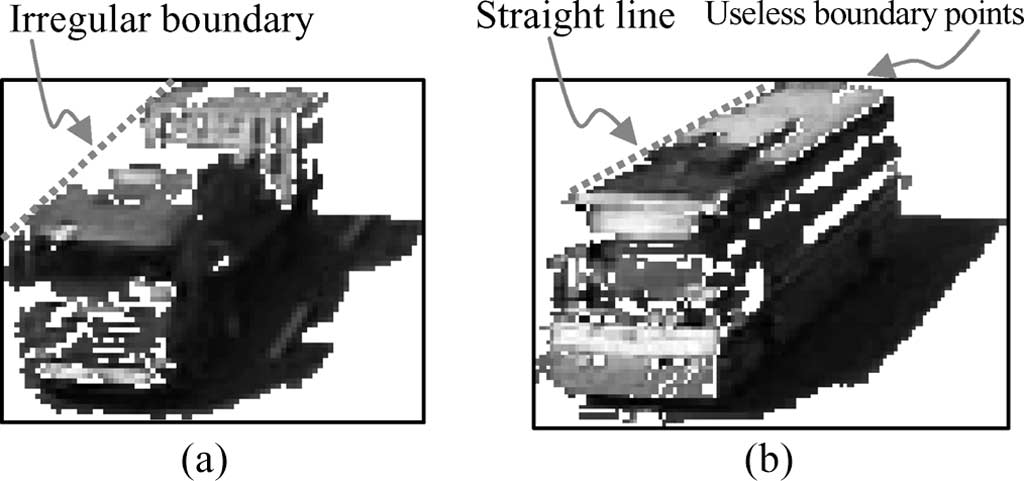
\includegraphics[width=3in]{linearity.png}
% where an .eps filename suffix will be assumed under latex, 
% and a .pdf suffix will be assumed for pdflatex; or what has been declared
% via \DeclareGraphicsExtensions.
\caption{Illustration by \cite{Jun-Wei}, showing the difference an irregular boundary of a truck (low linearity) and the straight line (high linearity) of a bus.}
\label{fig_linearity}
\end{figure}

To be able to acquire the linearity of a blob, first the set of up-slanted edges $U_{H_i}$ is acquired from the blob. However, because there are useless boundary points that will affect the linearity of the set of points, such as those found in figure~\ref{fig_linearity}b. The set must be filtered.

Given a set $U_{H_i}$, let the minimum bounding box be $B_{H_i}$. Let the distance of a point $q$ in the set $U_{H_i}$ to the bounding box be $d_{B_H} (q)$, and the maximum distance to the bounding box $d_{B_H}^{max} = max_{q \in U_{H_i}} \lbrace d_{B_{H_i}} (q) \rbrace $. The filtered set $\overline{U}_{H_i}$ is defined as:

$$
\overline{U}_{H_i} = \lbrace p \thinspace | \thinspace p \in U_{H_i} \thinspace , \thinspace d_{B_H}(p) > 0.25 d_{B_H}^{max} \thinspace \thinspace \rbrace
$$

The filtered set $\overline{U}_{H_i}$ is the set of points in $U_{H_i}$ that is at least 25\% of the maximum distance $d_{B_H}^{max}$. The above equation is an reduction of \cite{Jun-Wei}'s definition of the the filtered set, which initially had another condition to filter pixels that have a high probability of being a shadow.


Using the points in the set $\overline{U}_{H_i}$, the error function below is minimized \cite{Math}:

$$
E(b, m) = \sum_{i=1}^{N}(y_i - b_k - m_k x_i)^2
$$

The values of $m$ and $b$ can be acquired by:

$$
m_k = \frac{1}{K} \left( N \thinspace \bar{X} \thinspace \bar{Y} - \sum_{i=1}^{N} x_i \thinspace y_i \right)
$$

$$
b_k = \frac{1}{K} \left( \bar{X} \thinspace \sum_{i=1}^{N} x_i \thinspace y_i - \bar{Y} \sum_{i=1}^{N} x_i^2 \right)
$$

where $\bar{X}$, $\bar{Y}$, and $K$ are the following:

$$
\bar{X} = \frac{1}{N} \left( \sum_{i=1}^{N} x_i \right)
$$

$$
\bar{Y} = \frac{1}{N} \left( \sum_{i=1}^{N} y_i \right)
$$

$$
K = N \thinspace \bar{X} \thinspace \bar{X} - \sum_{i=1}^{N} x_i^2
$$

A vehicle with its up-slanted edges such as that of figure~\ref{fig_linearity}b will have very minimal error when it is plotted on the straight line model. This means that $E(b,m)$ will have a value closer to 0. However, a vehicle with an irregular boundary such as figure~\ref{fig_linearity}a will have points that will not fit in a line perfectly. This means that there is significant error; $E(b,m)$ will have a value farther from 0.

\cite{Jun-Wei} defines the linearity of a vehicle $H$ as:

$$
Linearity(H) = exp \left( \thinspace - \sqrt{\frac{1}{N} \thinspace \sum_{i=1}^{N} \thinspace (y_i - m x_i - b)^2 } \thinspace \right)
$$

By using the $exp$ function, the linearity values of a vehicle is bounded between 0 (high error) and 1 (minimal to no error).


\subsection{Vehicle classification}

This research classifies vehicles into 6 classes: sedan, bus, jeep, truck, SUV, and others.  \cite{Jun-Wei} classifies vehicles based on a vehicle template library. A template has the values of the features (size and linearity) and the corresponding vehicle classification. 
\begin{table}[]
\centering
\caption{Template instances per class}
\label{template_instances}
\begin{tabular}{|l|l|l|l|l|l|l|}
\hline
       & Sedans & Bus & Jeeps & Trucks & SUVs & Others \\ \hline
Count  & 250    & 52  & 53    & 14     & 238  & 153    \\ \hline
\end{tabular}
\end{table}

Table~\ref{template_instances} shows the number of template instances per class in the vehicle template library. A limitation in the dataset is the minimal templates available for instances of trucks, jeeps, and buses..

To classify a vehicle, the mean and the variance of the templates within a vehicle class $VC_k$ is acquired. Given the $j$th template $V_j^k$ of vehicle class $k$, the mean of the $r$th feature is defined as:

$$
m_k^r = \frac{1}{n_k} \thinspace \sum_{i=1}^{n_k} f_r (V_i^k)
$$

and the variance of the $r$th feature is defined as:

$$
\sigma_{r,k} = \sqrt{ \frac{1}{n_k} \thinspace \sum_{j=1}^{n_k} ( \thinspace f_r (V_j^k) - m_r^k \thinspace ) ^2 }
$$

Given a vehicle $H_i$ and a template $V_j^k$ in the vehicle classification $VC_k$, the similarity between the vehicle and the template is:

$$
S_k (H_i, V_j^k) = exp \left( \thinspace - \sum_{r=1}^{2} \frac{ (f_r(H_i) - f_r(V_j^k) )^2 }{\sigma_{r, k}^2 } \thinspace \right)
$$

The similarity of a vehicle $H_i$ to the whole vehicle class $VC_k$ is defined as:

$$
S_k (H_i | VC_k) = \frac{1}{n_k} \thinspace \sum_{V_j^k \in VC_k } S_k (H_i, V_j^k)
$$

The probability of the vehicle $H_i$ to be classified as vehicle class $VC_k$ is the similarity to the class $k$ over the total sum of similarities to all of the classes:

$$
P(VC_k | H_i) = \frac{S(H_i | VC_k)}{S_{sum} (H_i)}
$$


The classification given to a vehicle $H_i$ is the class with the highest probability. This system assigns the classification to a tracked vehicle after the vehicle has been tracked for more than 20 frames and has passed a certain horizontal line on the road, denoting that the blob's Y position has changed from state A (far in the distance) to state B (closer to the camera).

\section{Results}

The performance evaluation of the vehicle classification and counting is recorded using the EDSA dataset which contains 3567 frames. The total number of vehicles counted by the system was 111 vehicles, while the actual number of vehicles is 105.

Table~\ref{cm:sedan} to Table~\ref{cm:others} shows the confusion matrices of each of the classifiers. This is presented in the Figure~\ref{fig_classifier_performance} as an overview of classifier performances.

\begin{figure}[!ht]
\centering
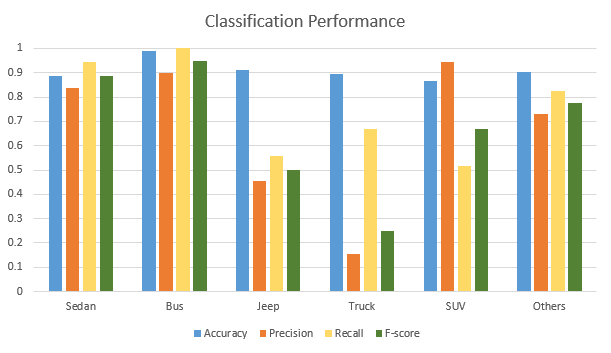
\includegraphics[width=3in]{classification_performance.png}
\caption{Accuracy, precision, recall performance of classifiers}
\label{fig_classifier_performance}
\end{figure}

The results showed good performance for tracking sedans and other vehicles but did not perform as well on the other classes such as buses, jeeps, trucks, and SUVs. This may be attributed to the low number of template instances for jeeps, trucks, and SUVs encoded into the vehicle template library as seen in table~\ref{template_instances}. The low number of encoded template instances was directly affected by the low number of vehicles that were actually in the dataset, seen in Table~\ref{cm:jeep} to Table~\ref{cm:suv}.

\begin{figure}[!ht]
\centering
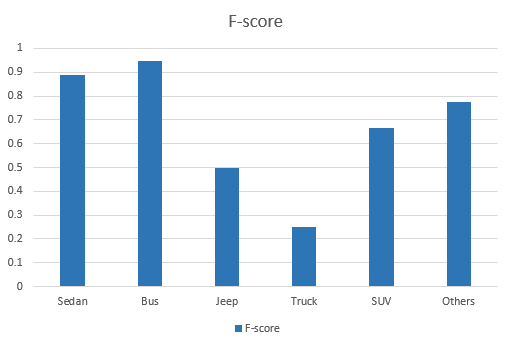
\includegraphics[width=3in]{Fscore.png}
\caption{F score performance of classifiers}
\label{fig_fscore_performance}
\end{figure}

Figure~\ref{fig_fscore_performance} shows the F-score performance of the classifiers. The results show that only Sedan, Bus, and Others had an F-score that is above 0.70. Trucks had a lower F-score because it had a low recall and precision of 66.67\% and 15.38\% respectively. 

\begin{figure}[!ht]
\centering
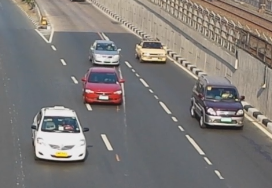
\includegraphics[width=3in]{occlusion.png}
\caption{Vehicle occlusion greatly affects bus classification}
\label{fig_occlusion}
\end{figure}

One of the causes of incorrectly classified buses is the inherent problem of occlusion in computer vision which is not part of the scope of this research. As seen in figure~\ref{fig_occlusion}, vehicles near each other may cause the segmentation process to incorrectly detect separate vehicles as connected blobs. This greatly affects bus classification which highly relies on its size feature.


\begin{table}[]
\centering
\caption{Sedan classification confusion matrix}
\label{cm:sedan}
\begin{tabular}{|c|c|c|c|}
\hline
\multicolumn{2}{|c|}{\multirow{2}{*}{Sedan}} & \multicolumn{2}{c|}{Prediction} \\ \cline{3-4} 
\multicolumn{2}{|c|}{}                       & False          & True           \\ \hline
\multirow{2}{*}{Actual}         & False      & 50             & 10             \\ \cline{2-4} 
                                & True       &  3             & 51             \\ \hline
\end{tabular}
\end{table}

The Sedan classifier had an accuracy rate of 88.60\%, recall of 94.44\%, and precision of 83.61\%. Its error rate was 11.40\% with specificity of 83.33\%. 

\begin{table}[]
\centering
\caption{Bus classification confusion matrix}
\label{cm:bus}
\begin{tabular}{|c|c|c|c|}
\hline
\multicolumn{2}{|c|}{\multirow{2}{*}{Bus}} & \multicolumn{2}{c|}{Prediction}  \\ \cline{3-4} 
\multicolumn{2}{|c|}{}                       & False          & True          \\ \hline
\multirow{2}{*}{Actual}         & False      & 101            & 1             \\ \cline{2-4} 
                                & True       & 0              & 9             \\ \hline
\end{tabular}
\end{table}

The Bus classifier had an accuracy rate of 99.10\%, recall of 100\%, and precision of 90\%. Its error rate was 0.90\% with specificity of 99.02\%. 

\begin{table}[]
\centering
\caption{Jeep classification confusion matrix}
\label{cm:jeep}
\begin{tabular}{|c|c|c|c|}
\hline
\multicolumn{2}{|c|}{\multirow{2}{*}{Jeep}} & \multicolumn{2}{c|}{Prediction} \\ \cline{3-4} 
\multicolumn{2}{|c|}{}                       & False          & True           \\ \hline
\multirow{2}{*}{Actual}         & False      & 98             & 11             \\ \cline{2-4} 
                                & True       &  1             &  2             \\ \hline
\end{tabular}
\end{table}

The Jeep classifier had an accuracy rate of 91.30\%, recall of 55.56\%, and precision of 45.45\%. Its error rate was 8.70\% with specificity of 94.34\%. 

\begin{table}[]
\centering
\caption{Truck classification confusion matrix}
\label{cm:truck}
\begin{tabular}{|c|c|c|c|}
\hline
\multicolumn{2}{|c|}{\multirow{2}{*}{Truck}} & \multicolumn{2}{c|}{Prediction} \\ \cline{3-4} 
\multicolumn{2}{|c|}{}                       & False          & True           \\ \hline
\multirow{2}{*}{Actual}         & False      & 98             & 11             \\ \cline{2-4} 
                                & True       &  1             &  2             \\ \hline
\end{tabular}
\end{table}

The Truck classifier had an accuracy rate of 89.29\%, recall of 66.67\%, and precision of 15.38\%. Its error rate was 10.71\% with specificity of 89.91\%. 

\begin{table}[]
\centering
\caption{SUV classification confusion matrix}
\label{cm:suv}
\begin{tabular}{|c|c|c|c|}
\hline
\multicolumn{2}{|c|}{\multirow{2}{*}{SUV}} & \multicolumn{2}{c|}{Prediction} \\ \cline{3-4} 
\multicolumn{2}{|c|}{}                       & False          & True           \\ \hline
\multirow{2}{*}{Actual}         & False      & 93             &  1              \\ \cline{2-4} 
                                & True       & 16             & 17             \\ \hline
\end{tabular}
\end{table}

The Sedan classifier had an accuracy rate of 86.61\%, recall of 51.52\%, and precision of 94.44\%. Its error rate was 13.39\% with specificity of 98.94\%. 

\begin{table}[]
\centering
\caption{Others classification confusion matrix}
\label{cm:others}
\begin{tabular}{|c|c|c|c|}
\hline
\multicolumn{2}{|c|}{\multirow{2}{*}{Others}} & \multicolumn{2}{c|}{Prediction} \\ \cline{3-4} 
\multicolumn{2}{|c|}{}                       & False          & True           \\ \hline
\multirow{2}{*}{Actual}         & False      & 85             &  7              \\ \cline{2-4} 
                                & True       &  4             & 19             \\ \hline
\end{tabular}
\end{table}

The Others classifier had an accuracy rate of 90.43\%, recall of 82.61\%, and precision of 73.08\%. Its error rate was 9.57\% with specificity of 92.39\%. 


Figure~\ref{fig_template_visualization} shows a visualization of the instances in the vehicle template library, showing the size (y axis) and the linearity (x axis) of the instances and colored by class. 

\begin{figure}[!ht]
\centering
% 
\includegraphics[width=2.5in]{myfigure}
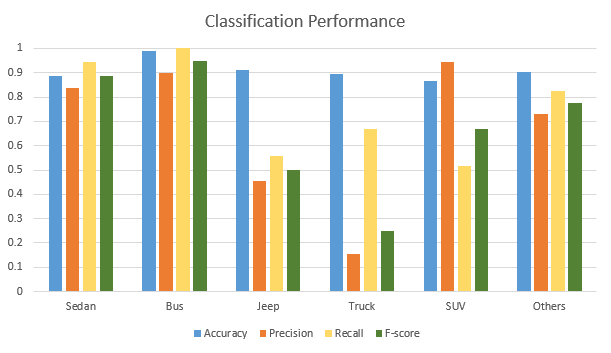
\includegraphics[width=3in]{classification_performance.png}
% where an .eps filename suffix will be assumed under latex, 
% and a .pdf suffix will be assumed for pdflatex; or what has been declared
% via \DeclareGraphicsExtensions.
\caption{An excerpt of the visualization plotting the clustering of instances in the vehicle template library. }
\label{fig_template_visualization}
\end{figure}

The visualization shows the high variance in the features of sedan instances (green) as seen in their varying sizes. Bus instances (blue) were distant from the main cluster and are easily discriminated by their large size. Two clusters of the other instances (red) can easily be seen: one that clusters around $size = 1$ which is interpreted to be van instances, and one that clusters around $size = 0.25$ which is interpreted to be motorcycle instances. With the number of vehicle instances in the dataset for SUVs (orange), trucks (gray), and jeeps(yellow), the results show that their size and linearity features are clustered together and are not yet sufficient for classification.


% Note that IEEE does not put floats in the very first column - or typically
% anywhere on the first page for that matter. Also, in-text middle ("here")
% positioning is not used. Most IEEE journals use top floats exclusively.
% Note that, LaTeX2e, unlike IEEE journals, places footnotes above bottom
% floats. This can be corrected via the \fnbelowfloat command of the
% stfloats package.

\section{Conclusion}

This research was able to collect and analyze vehicle datasets, to identify common problems in vehicle traffic datasets in the context of the Philippines, and to implement a variation of \cite{Jun-Wei}'s vehicle identification and classification system. Results of the classification and the visualization of the vehicle template library confirm that sedan and motorcycle classification shows promising clustering results. The main challenge of bus classification is the problem of occlusion, while other classes (jeep, truck, SUVs) require more data instances to improve the classification or more blob/vehicle features to be introduced.

Noise in vehicle traffic dataset include occlusion problems caused by electrical wires. A challenge in background modeling is the common occurrence for vehicles such as jeeps, buses, and shuttles to park either because they are boarding or alighting passengers or because of traffic stop-lights. Also, the dataset shows that there are vehicles that park in the middle of two lanes, for as long as twenty seconds just to board, alight, and wait for passengers. 

\section{Recommendations}

Various improvements can be made with this research. A larger dataset can be collected and more instances encoded in the vehicle template library to improve the performance of the vehicle classification approach. Future works can study other properties of blobs (such as convexity) to see if there are other features that can be used aside from size and linearity. Vehicle classification under different settings such as varying weather conditions (sunny, rainy, cloudy) or varying traffic conditions (traffic stand-still) can be explored. The main algorithm for vehicle detection and classification will need to adapt when performed on a dataset that has heavy stand-still traffic, because the background modeling approach used in this research will not be as effective on slow or non-moving vehicles. 

\clearpage

\appendices
\section{Class Instances of the Vehicles}

Figures~\ref{fig_sedan} to \ref{fig_van} show instances of the classes found in the EDSA dataset.

\begin{figure}[!h]
\centering
% 
\includegraphics[width=2.5in]{myfigure}
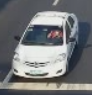
\includegraphics{vehicle_sedan.png}
% where an .eps filename suffix will be assumed under latex, 
% and a .pdf suffix will be assumed for pdflatex; or what has been declared
% via \DeclareGraphicsExtensions.
\caption{A sedan is the car type that is most common in the dataset, with low height and is often used by taxis. Example of these are Toyota Altis, Vios, etc.}
\label{fig_sedan}
\end{figure}

\begin{figure}[!h]
\centering
% 
\includegraphics[width=2.5in]{myfigure}
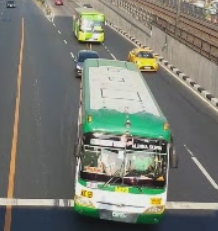
\includegraphics{vehicle_bus.png}
% where an .eps filename suffix will be assumed under latex, 
% and a .pdf suffix will be assumed for pdflatex; or what has been declared
% via \DeclareGraphicsExtensions.
\caption{Buses in the Philippines are long, tall, and wide. They occupy almost the whole space  on a lane.}
\label{fig_bus}
\end{figure}

\begin{figure}[!h]
\centering
% 
\includegraphics[width=2.5in]{myfigure}
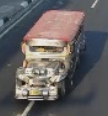
\includegraphics{vehicle_jeep.png}
% where an .eps filename suffix will be assumed under latex, 
% and a .pdf suffix will be assumed for pdflatex; or what has been declared
% via \DeclareGraphicsExtensions.
\caption{Jeeps or Jeepneys are vehicles that are long with average height. These vehicles stop on the side of the road to alight and pick up passengers. The reflection of the sunlight on the road reflected from the metal casing of the jeep is sometimes recognized by the segmentation module.}
\label{fig_jeep}
\end{figure}

\begin{figure}[!h]
\centering
% 
\includegraphics[width=2.5in]{myfigure}
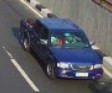
\includegraphics{vehicle_truck.png}
% where an .eps filename suffix will be assumed under latex, 
% and a .pdf suffix will be assumed for pdflatex; or what has been declared
% via \DeclareGraphicsExtensions.
\caption{The distinguising feature of trucks is their rear luggage space that can carry equipment or large objects. Trucks aren't as common in the third dataset. Industry or delivery trucks of companies were not found in the dataset.}
\label{fig_truck}
\end{figure}

\begin{figure}[!h]
\centering
% 
\includegraphics[width=2.5in]{myfigure}
\includegraphics{vehicle_suv.png}
% where an .eps filename suffix will be assumed under latex, 
% and a .pdf suffix will be assumed for pdflatex; or what has been declared
% via \DeclareGraphicsExtensions.
\caption{Sports utility vehicles (SUVs) are larger than sedans and usually have mechanisms on the top of the vehicle for carrying equipment. Examples of these are Fortuner, Montero Sport, CRV, etc.}
\label{fig_suv}
\end{figure}

\begin{figure}[!h]
\centering
% 
\includegraphics[width=2.5in]{myfigure}
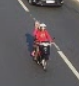
\includegraphics{vehicle_motorcycle.png}
% where an .eps filename suffix will be assumed under latex, 
% and a .pdf suffix will be assumed for pdflatex; or what has been declared
% via \DeclareGraphicsExtensions.
\caption{Motorcycles were found in the dataset, although bicycles and scooters were not found. These vehicles fall under the \textit{others} category.}
\label{fig_motorcycle}
\end{figure}


\begin{figure}[!h]
\centering
% 
\includegraphics[width=2.5in]{myfigure}
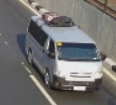
\includegraphics{vehicle_van.png}
% where an .eps filename suffix will be assumed under latex, 
% and a .pdf suffix will be assumed for pdflatex; or what has been declared
% via \DeclareGraphicsExtensions.
\caption{Vans are long vehicles, that can carry more passengers than sedans. These vehicles fall under the \textit{others} category.}
\label{fig_van}
\end{figure}

% use section* for acknowledgement
\section*{Acknowledgment}

The author would like to thank Dr. Joel Ilao of the College of Computer Studies, De La Salle University, Manila for his contribution as the adviser on this research project.


% Can use something like this to put references on a page
% by themselves when using endfloat and the captionsoff option.
\ifCLASSOPTIONcaptionsoff
  \newpage
\fi



% trigger a \newpage just before the given reference
% number - used to balance the columns on the last page
% adjust value as needed - may need to be readjusted if
% the document is modified later
%\IEEEtriggeratref{8}
% The "triggered" command can be changed if desired:
%\IEEEtriggercmd{\enlargethispage{-5in}}

% references section

% can use a bibliography generated by BibTeX as a .bbl file
% BibTeX documentation can be easily obtained at:
% http://www.ctan.org/tex-archive/biblio/bibtex/contrib/doc/
% The IEEEtran BibTeX style support page is at:
% http://www.michaelshell.org/tex/ieeetran/bibtex/
%\bibliographystyle{IEEEtran}
% argument is your BibTeX string definitions and bibliography database(s)
%\bibliography{IEEEabrv,../bib/paper}
%
% <OR> manually copy in the resultant .bbl file
% set second argument of \begin to the number of references
% (used to reserve space for the reference number labels box)
\begin{thebibliography}{1}

\bibitem{Jun-Wei}
Jun-Wei Hsieh, Shih-Hao Yu, Yung-Sheng Chen and Wen-Fong Hu, "Automatic traffic surveillance system for vehicle tracking and classification," in IEEE Transactions on Intelligent Transportation Systems, vol. 7, no. 2, pp. 175-187, June 2006.

\bibitem{Sobral}
Sobral, Andrews. BGSLibrary: An OpenCV C++ Background Subtraction Library. IX Workshop de Visão Computacional (WVC'2013), Rio de Janeiro, Brazil, Jun. 2013.

\bibitem{Math}
W. H. Press, S. A. Teukolsky, W. T. Vetterling, and B. P. Flannery, Numerical Recipes in C—The Art of Scientific Computing. Cambridge, U.K.: Cambridge Univ. Press, 1992.

\bibitem{Manzanera}
Antoine Manzanera and Julien C. Richefeu. A new motion detection algorithm based on Σ-Δ background estimation. Pattern Recognition Lett. 28, 3 (February 2007), p. 320-328.
\end{thebibliography}

% biography section
% 
% If you have an EPS/PDF photo (graphicx package needed) extra braces are
% needed around the contents of the optional argument to biography to prevent
% the LaTeX parser from getting confused when it sees the complicated
% \includegraphics command within an optional argument. (You could create
% your own custom macro containing the \includegraphics command to make things
% simpler here.)
%\begin{biography}[{\includegraphics[width=1in,height=1.25in,clip,keepaspectratio]{mshell}}]{Michael Shell}
% or if you just want to reserve a space for a photo:

\begin{IEEEbiography}[{\includegraphics[width=1in,height=1.25in,clip,keepaspectratio]{picture}}]{John Doe}
\blindtext
\end{IEEEbiography}


\vfill

% Can be used to pull up biographies so that the bottom of the last one
% is flush with the other column.
\enlargethispage{-5in}



\end{document}


